\documentclass{article}
\usepackage{titlesec}
\usepackage{verbatim}
%provides multi-line comment syntax : \begin{comment} \end{comment}
\usepackage{xeCJK}
\usepackage[xetex]{graphicx}


\begin{comment}
\titleformat{\section}[runin]
  {\normalfont\Large\bfseries}{\thesection}{1em}{}
\end{comment}
\titleformat{\subsection}[runin]
  {\normalfont\large\bfseries}{\thesubsection}{1em}{}
\titleformat{\subsubsection}[runin]
  {\normalfont\large\bfseries}{\thesubsection}{1em}{}

\title{OS project 1}
\author{R05922092 張耿健, B04902045 孫凡耘}
\date{\today}

\begin{document}
\maketitle

    \section{Implementation Details}
        Environment: Oracle VM VirtualBox, version: 5.1.16\newline
        I followed similar steps described in the PPT when I build the kernel.\newline
        Implementation steps:
        \subsection*{1.}
            Add system call to the system call table.
        \subsection*{2.}
            Add macro \#define \_\_NR\_functionName xxx(my definition), update NR\_SYSCALLS accordingly.
        \subsection*{3.}
            Add prototype of the system call with a prefix sys\_ at syscalls.h.
        \subsection*{4.}
            Modify Makefile, add functionName.o to obj-y.
        \subsection*{5.}
            Rebuild and Reboot into the kernel that I just compiled, then run my test program using syscall(\_\_NR\_functionName, Parameters).

    \section{Faced Difficulties}
        Implementing show, min, and multiply is pretty simple. But the true difficulty comes when we try to implent CPU\_Utilization.\newline
        \subsection*{1.} Many simple operations that we are familiar with cannot be directly used in Kernel Space environment. For example, the use of FILE * or the arithmetic of floating point numbers, so we'll have to look up special functions or procedures to deal with it.
        \subsection*{2.} A big difficulty when implementing the system calls is that everytime we made a typo or silly mistake, it takes us a long time to figure it out since compiling the kernel is time-consuming. So I learned to code more carefully and double check for syntax errors before I recompile my kernel.
        \subsection*{3.} I found out that the result of my CPU\_Utilization is 100\%. At first, I thought this is unreasonable. But at last, I found out that it's not my problem. The CPU Utilization is indeed 100\% on the virtual machine( the CPU is always utilized by user and system ). I double checked it with top command and cat /proc/stat( the idle time, which is the fourth parameter,  is not changing).
        \begin{figure}[!htb]
            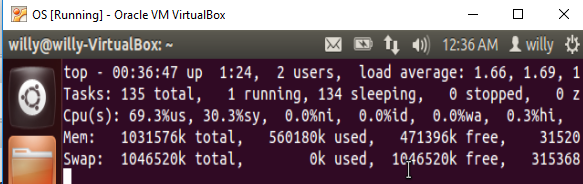
\includegraphics[scale=0.4]{top.png}
        \end{figure}

    \section{Results}
            \begin{verbatim}
// test min and multiply
printf("8*7 = %d\n", syscall(339, 8, 7));
printf("min(100, 1) = %d\n", syscall(340, 100, 1));
// test hello, check from dmesg
syscall(337);
//test show, check from dmesg
syscall(338);
//test CPU_Utilization(show percentage), check from dmesg
syscall(341);
            \end{verbatim}
            \begin{figure}[!htb]
                \begin{flushleft}
                    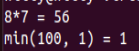
\includegraphics[scale=0.7]{result1.png}
                \end{flushleft}
            \end{figure}
            \begin{figure}[!htb]
                \begin{flushleft}
                    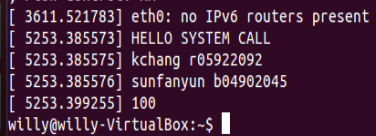
\includegraphics[scale=0.4]{result2.png}
                \end{flushleft}
            \end{figure}



\end{document}
